\chapter{Implementacja programowa oraz sprzętowa wybranej architektury sieci}
\label{cha:Implementacja}
% Opis oraz omówienie implementacji zarówno programowej jak i sprzętowej.

Opracowanie odpowiedniej architektury sieci oprócz rozważań teoretycznych, wymagało również wykonania szeregu eksperymentów obliczeniowych.
Ponadto konieczna była również implementacja sprzętowa modelu celem akceleracji obliczeń zaprojektowanej architektury.

\section{Implementacja programowa}

Implementacja programowa została zrealizowana w ramach framework'a \emph{PyTorch} \cite{pytorch}.
Wykorzystano również bibliotekę \emph{Brevitas} \cite{brevitas} do realizacji odpowiedniej metody kwantyzacji, która polegała na zdefiniowaniu klasy o parametrach statycznych definiujących zachowanie się obiektu. 
Metodyka implementacji kwantyzacji opiera się o klasę \emph{ExtendedInjector}.
Pozwala ona na ``wstawienie'' operacji kwantyzacji wag bezpośrednio przed zastosowaniem ich w obliczeniach.
Ponadto biblioteka rozszerza predefiniowane w \emph{PyTorch} warstwy o operacje kwantyzacji. 
W wersji kwantyzowanej dostępne są m.in. warstwa konwolucji, \emph{Max Pooling} czy funkcja $ReLU$.
Kwantyzowana warstwa normalizacji została zdefiniowana jako przekształcenie afiniczne bez aproksymacji średniej i wariancji.
Wymagało to implementacji własnej warstwy dokonującej wyboru pomiędzy warstwą zmiennoprzecinkową oraz jej wersją kwantyzowaną.
Augmentacja danych została zrealizowana w oparciu o bibliotekę \emph{OpenCV} \cite{opencv}.
Obliczenia były wykonywane na platformie \emph{GoogleColab} \cite{colab} z wykorzystaniem \emph{GPU}.
Ze względu, iż dzienny czas użytkowania usługi jest ograniczony wymagane było przechowywanie stanu procesu ucznia w plikach zapisywanych poprzez usługę \emph{GoogleDrive}.

Dla celu testowania wyników implementacji sprzętowej został zaimplementowany również model programowy odpowiednich warstw z wykorzystaniem obliczeń całkowitoliczbowych oraz mechanizm inicjalizacji wag modelu sprzętowego.

\section{Implementacja sprzętowa}
Wstępnie planowano implementacje sprzętową z wykorzystaniem narzędzia \emph{FINN} \ref{ch:tools}.
Jednakże ze względu na braki w dokumentacji zdecydowano się na implementację własną początkowo w języku \emph{HLS}, lecz ostatecznie w języku \emph{System Verilog}.
Akceleracja całej sieci stanowi architekturę potokową gruboziarnistą (ang. \emph{coarse grained}).
Schemat przedstawiono na rysunku \ref{fig:LNACC}.
Na elementy wspomnianej architektury składają się bloki pamięci RAM oraz ROM, multipleksery dostępu do pamięci, akceleratory poszczególnych warstw oraz logika sterująca (\emph{LN\_CU}, ang. \emph{LittlNet Control Unit}).
Wykorzystywana jest tutaj komunikacja z wykorzystaniem protokołu \emph{AXI4-Stream} \cite{axis} do komunikacji z \emph{DMA} (ang. \emph{Direct Memory Access}) \cite{dma}.
Wymiana danych odbywa się za pośrednictwem  modułów \emph{AXIS RECEIVER} do odbioru oraz \emph{AXIS SENDER} do wysyłania danych zgromadzonych w rejestrze \emph{SPR} (ang. \emph{Serial-Parallel Register}).
Poszczególne akceleratory pogrupowane są w bloki po 3 akceleratory. 
Na jeden blok przypisane są dwa bloki pamięci RAM, w tym jeden z dostępem  multipleksowanym.
Ostatnia warstwa wyznacza parametry obiektu zajmujące 7 bajtów.
Z tego względu dane te są umieszczone w rejestrze \emph{SPR} (zamiast w pamięci RAM).
Proces akceleracji odbywa się według schematu prezentowanego w tabeli \ref{tab:LNACC}
W jednej chwili są aktywne akceleratory co czwartej warstwy.
Jest to wymagane, aby udzielić dostępu do wybranych bloków pamięci kilku akceleratorom.

\begin{figure}
    \centering
    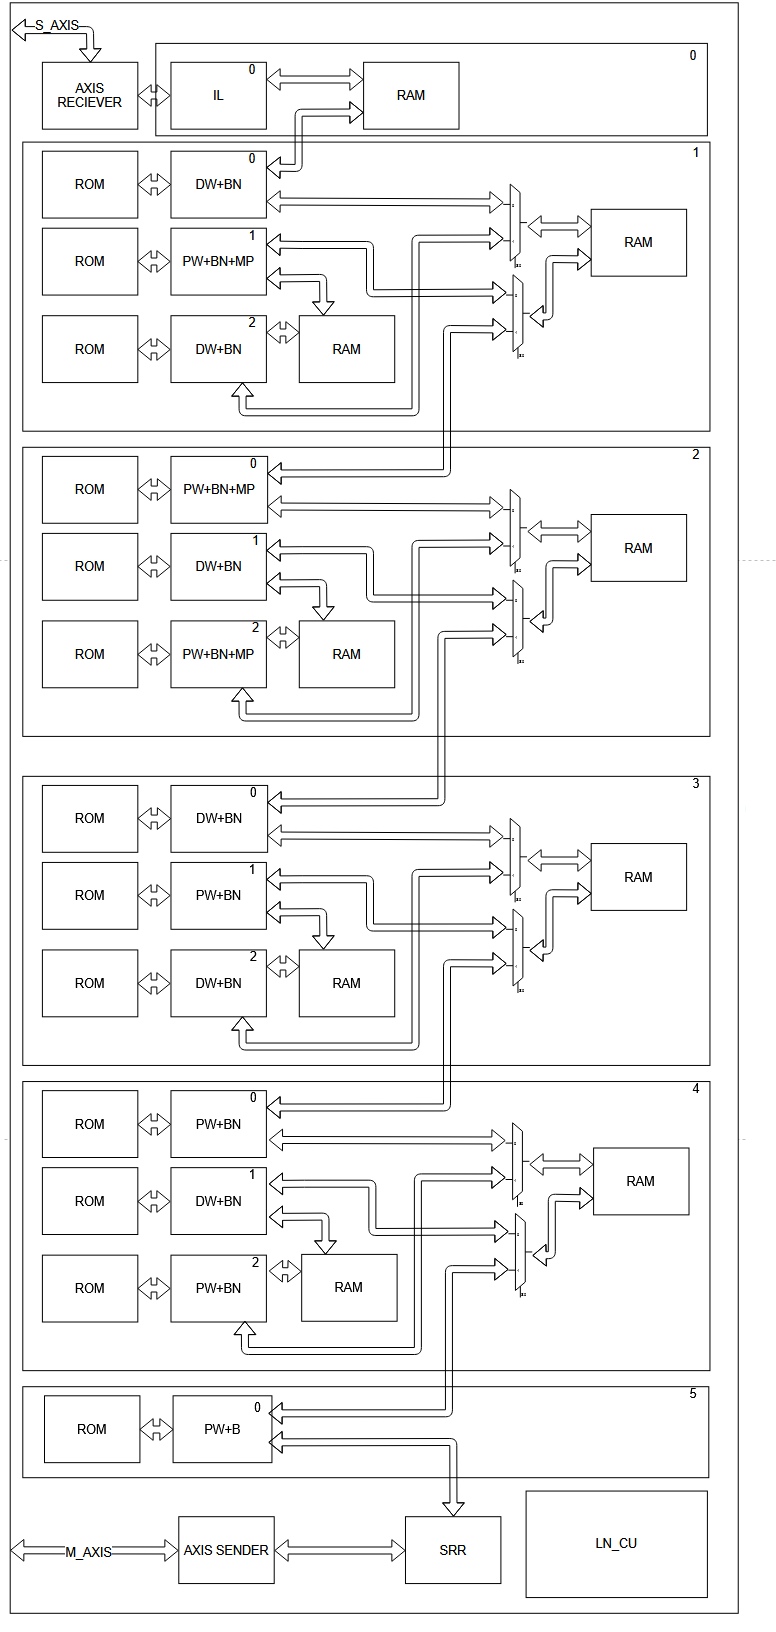
\includegraphics[height=0.9\textheight]{images/LNACC.png}
    \caption{Schemat akceleracji architektury \emph{LittleNet}. Uwzględniono jedynie najistotniejsze elementy.}
    \label{fig:LNACC}
\end{figure}
\begin{table}
    \centering
    \caption{Schemat aktywacji akceleratorów zrealizowany jako maszyna stanów.}
    \label{tab:LNACC}
    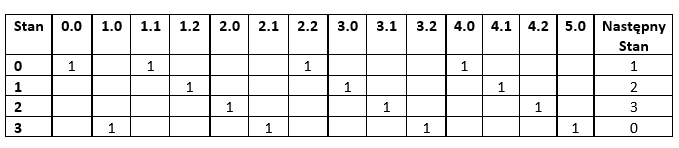
\includegraphics[width=0.9\textwidth]{images/acc_activ.png}
\end{table}

Wyróżniono 3 typy akceleratorów:
\begin{description}
\item warstwa wejściowa,
\item warstwa \emph{depthwise},
\item warstwa \emph{pointwise}.
\end{description}
Dostępnych w kilku konfiguracjach.

Ponadto zapis do pamięci wyjściowej w każdej warstwie jest zrealizowany przez moduł \emph{MWU} (ang. \emph{Memory Writer Unit}) przedstawiony na rysunku \ref{fig:mwu}.
Wykonuje on operacje analogiczne do rejestru równoległo-szeregowego.
Wejściowe równoległe $P$ kanałów $CH\_i$ zostają odpowiednio opóźnione. 
Każdy kanał $CH\_{i}$ przechodzi przez linię opóźniającą \emph{D} o latencji równej indeksowi sygnału $i$.
Do każdego kanału przypisany jest licznik adresu $CHD\_i$.
W przypadku, gdy opóźniona wartość kanału jest uznawana za ważną (ang. \emph{valid}) następuje inkrementacja adresu.
Wszystkie opóźnione kanały są multipleksowane wybierając kolejne kanały wraz z ich adresami.
Uzyskiwane sygnały stanowią interfejs pamięci docelowej.

\begin{figure}
    \centering
    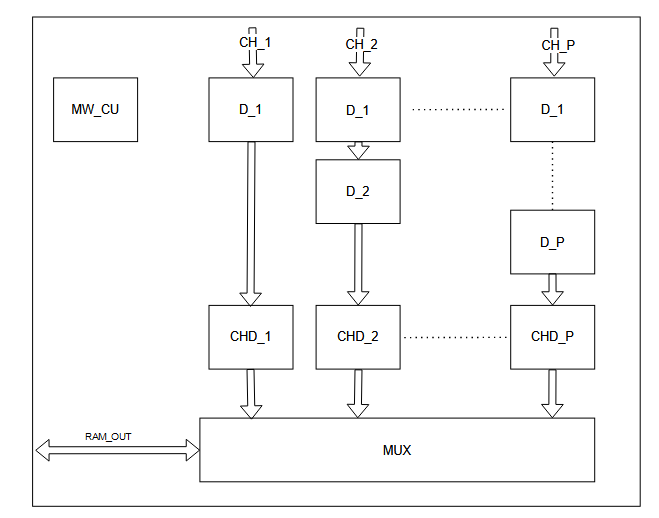
\includegraphics[width=0.8\linewidth]{images/MWU.png}
    \caption{\emph{MWU} - schemat generowania adresu dla przetwarzania wielokanałowego.}
    \label{fig:mwu}
\end{figure}

\subsection{Warstwa wejsciowa}
Warstwa wejściowa \emph{IL} (ang. \emph{Input Layer}) realizuje zadanie zmiany formatu danych.
Dane wejściowe otrzymywane są w notacji \emph{H-W-CH} (ang \emph{Height-Width-Channel}).
Na dalszym etapie przetwarzania wymagany jest format \emph{CH-H-W}.
Realizowane jest to poprzez buforowanie 3 kolejnych 32 bitowych pakietów danych w rejestrze szeregowo-równoległym.
Zgromadzone dane są rozdzielane na poszczególne składowe kanałów składając się na 32 bitowe pakiety po jednym na każdy kanał.
Jest zapisywany do pamięci poprzez moduł \emph{MWU} dla 3 kanałów.
Schemat akceleratora został przedstawiony na rysunku \ref{fig:il}.
\begin{figure}
    \centering
    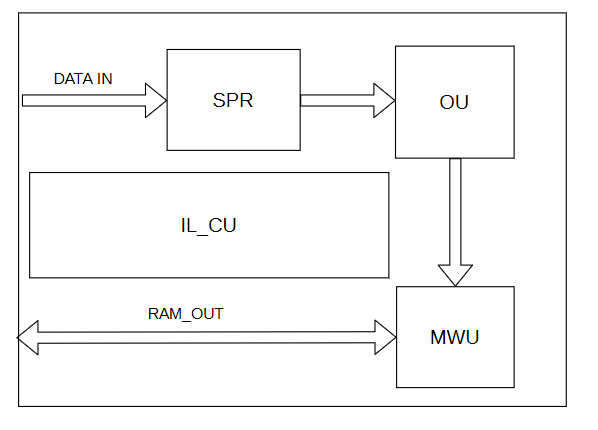
\includegraphics[width=0.8\linewidth]{images/ILACC.png}
    \caption{Schemat warstwy wejściowej \emph{IL}.}
    \label{fig:il}
\end{figure}

\subsection{Warstwa \emph{depthwise}}
Akceleracja konwolucji \emph{DW} jest realizowana razem z warstwą normalizującą.
Na rysunku \ref{fig:dwacc} przedstawiono schemat akceleratora \emph{DW}.
Obliczenia wykonywane są w architekturze potokowej drobnoziarnistej (ang. \emph{fine grained}). 
W tym celu moduł \emph{SWU} (ang. \emph{Sliding Window Unit}) generuje strumień danych wraz z odpowiednimi opóźnieniami tak, aby wygenerować kontekst okna przesuwnego o wymiarach 3x3.
Wykonanie operacji konwolucji wymaga wcześniejszego (przed rozpoczęciem strumienia każdego kanału) wczytania wag maski konwolucji.
Operację tę wykonuje moduł \emph{WSL} (ang. Weights Loading Unit).
Sama operacja iloczynu skalarnego wektora wag i kontekstu jest wykonywana przez \emph{DW\_PU} (ang. \emph{DepthWise Processing Unit}) przedstawiony na schemacie \ref{fig:dwpu}.
Wykorzystano tutaj możliwość kaskadowego połączenia kolejnych 9 \emph{DSP}. 
Możliwa jest konfiguracja z użyciem składowej bias (\emph{B}) oraz normalizacji poprzez przekształcenie afiniczne (\emph{BN}).
Wynik konwolucji oraz normalizacji jest ograniczany (\emph{LIMIT}) do wartości wynikających z wybranej notacji stałoprzecinkowej, czy też zastosowania funkcji $ReLU$.

Uzyskany rezultat jest zapisywany pod adresem wyznaczonym przez \emph{MWU}.
Sterowanie procesem odbywa się poprzez logikę reprezentowaną przez \emph{DW\_CU} (ang. \emph{DepthWise Control Unit}).
Wykonanie wielokrotnej konwolucji \emph{DW} odbywa się poprzez wielokrotne (cyliczne) generowanie strumienia danych wejściowych.
\begin{figure}
    \centering
    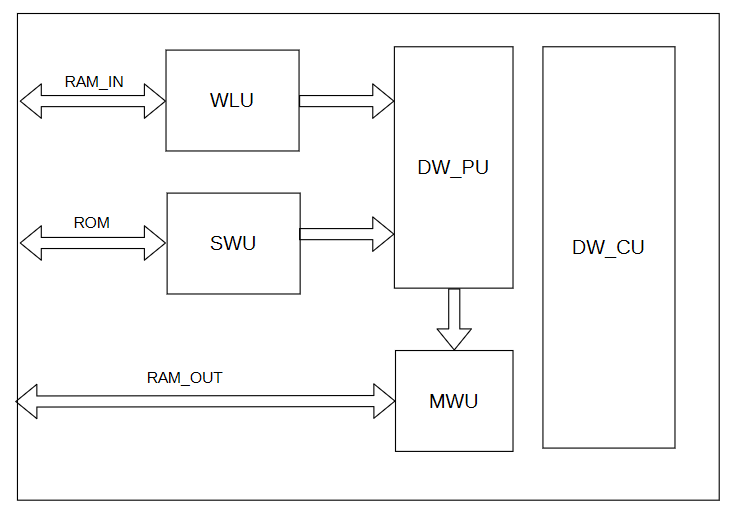
\includegraphics[width=0.9\linewidth]{images/DWACC.png}
    \caption{Schemat akceleratora \emph{DW} dostępnego w wielu konfiguracjach.}
    \label{fig:dwacc}
\end{figure}
\begin{figure}
    \centering
    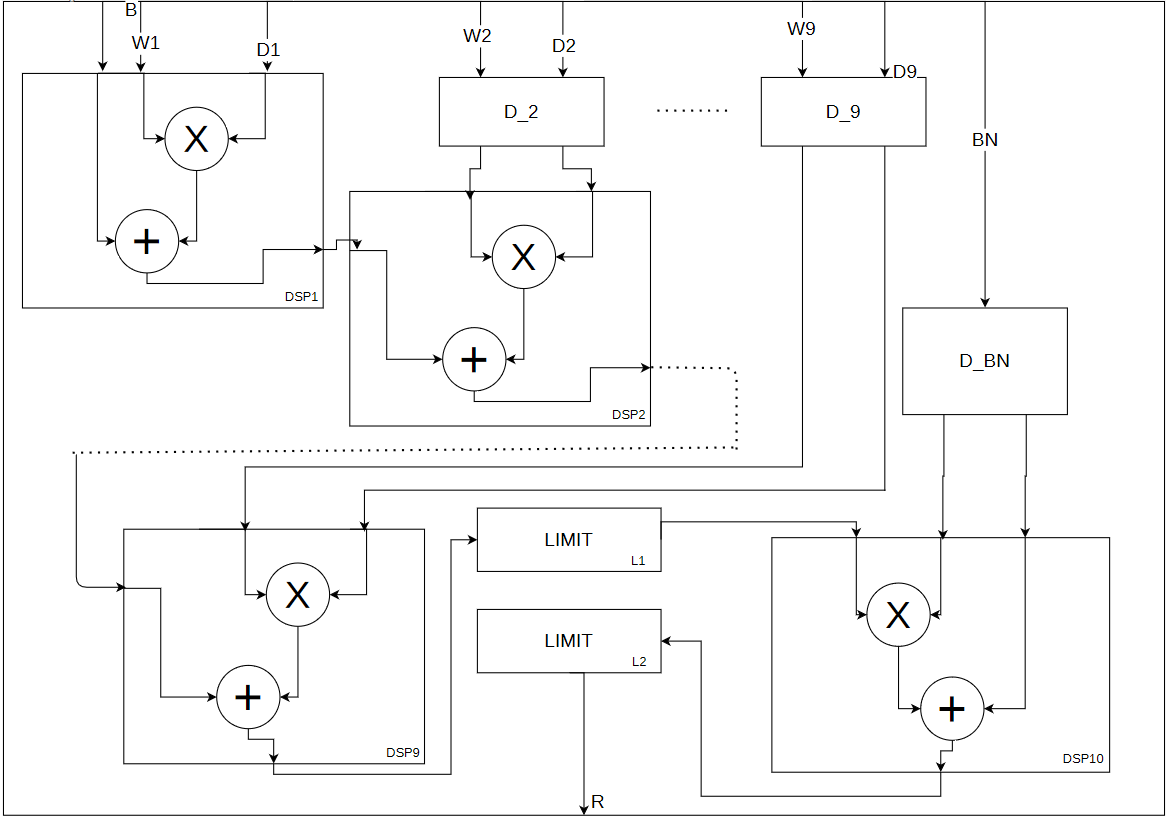
\includegraphics[width=0.9\linewidth]{images/DW_PU.png}
    \caption{Schemat \emph{DW\_PU} - kaskadowe połączenie \emph{DSP}.
    Bloki \emph{DSP10+L2} są opcjonalne zależnie od konfiguracji.}
    \label{fig:dwpu}
\end{figure}

\subsection{Warstwa \emph{pointwise}}
Podobnie jak w poprzednim przypadku akcelerator konwolucji \emph{PW} dostępny jest w wielu konfiguracjach.
Schemat akceleratora \emph{PW} prezentuje rysunek \ref{fig:pwacc}.
Operacja konwolucji \emph{PW} nie wymaga gromadzenia otoczenia rozpatrywanego punktu, lecz iterowania po kolejnych kanałach wejściowych w danym punkcie.
Jest to realizowane przez moduł \emph{PSU} (ang. \emph{Point Streamer Unit}).
Dla każdego kanału rozważanego punktu jest wymagana odpowiednia waga.
Ponadto identyczna sekwencja wag jest wymagana dla następnych puntów.
W tym celu moduł \emph{CSU} (ang. \emph{Cyclic Streamer Unit}) generuje strumień w sposób cykliczny.
Następuje wielokrotny odczyt z kolejnych adresów zadanej puli adresowej definiowanej przez liczbę wag filtru. 
Przed rozpoczęciem generowania strumienia wymagane jest jednak odczytanie wag bias oraz przekształcenia afinicznego wraz z ich przechowaniem w odpowiednich rejestrach.
Obliczenie konwolucji dla kolejnych punktów jest realizowane przez moduł \emph{PW\_PU} (ang. \emph{PointWise Processing Unit}) (rysunek \ref{fig:pwpu}).
Wykorzystuje się do tego celu operacje akumulacji z mnożeniem.
Zakumulowana suma iloczynów jest (zależnie od konfiguracji) powiększana o wartość bias.
Uzyskany rezultat zostaje ograniczony (tak jak konwolucji \emph{DW}).
W następnym kroku wykonywana jest operacja normalizacji wraz z ponownym ograniczeniem wartości.

Następnym etapem przetwarzania jest (ewentualna) operacja \emph{Max Pooling}.
Do tego celu wykorzystuje się odpowiednie opóźnienia oraz porównywania wartości.
Uzyskany rezultat jest zapisywany pod adresem wyznaczanym przez moduł \emph{MWU}.
Opcjonalną funkcjonalnością (dla warstwy \emph{YOLOv3}) jest zastąpienie \emph{MWU} przez \emph{MFU} (ang. \emph{Max Finder Unit}) pozwalającego znaleźć punkt o największej wartości wykrywalności obiektu, a także zwrócić jego parametry.
Ponadto istnieje możliwość zrównoleglenia obliczeń poprzez wykorzystanie $P$ modułów \emph{PW\_PU}. 

Sterowanie poszczególnymi modułami jest realizowane przez logikę reprezentowana przez \emph{PW\_CU} (ang. \emph{PointWise Control Unit}).

\begin{figure}
    \centering
    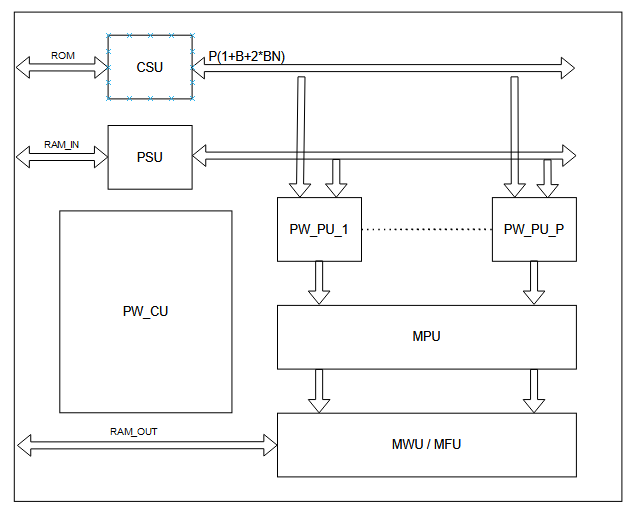
\includegraphics[width=0.9\linewidth]{images/PWACC.png}
    \caption{Schemat akceleratora \emph{PW} dostępnego w wielu konfiguracjach.
    Opcjonalne są moduły \emph{MPU} oraz \emph{MWU} lub \emph{MFU}.}
    \label{fig:pwacc}
\end{figure}
\begin{figure}
    \centering
    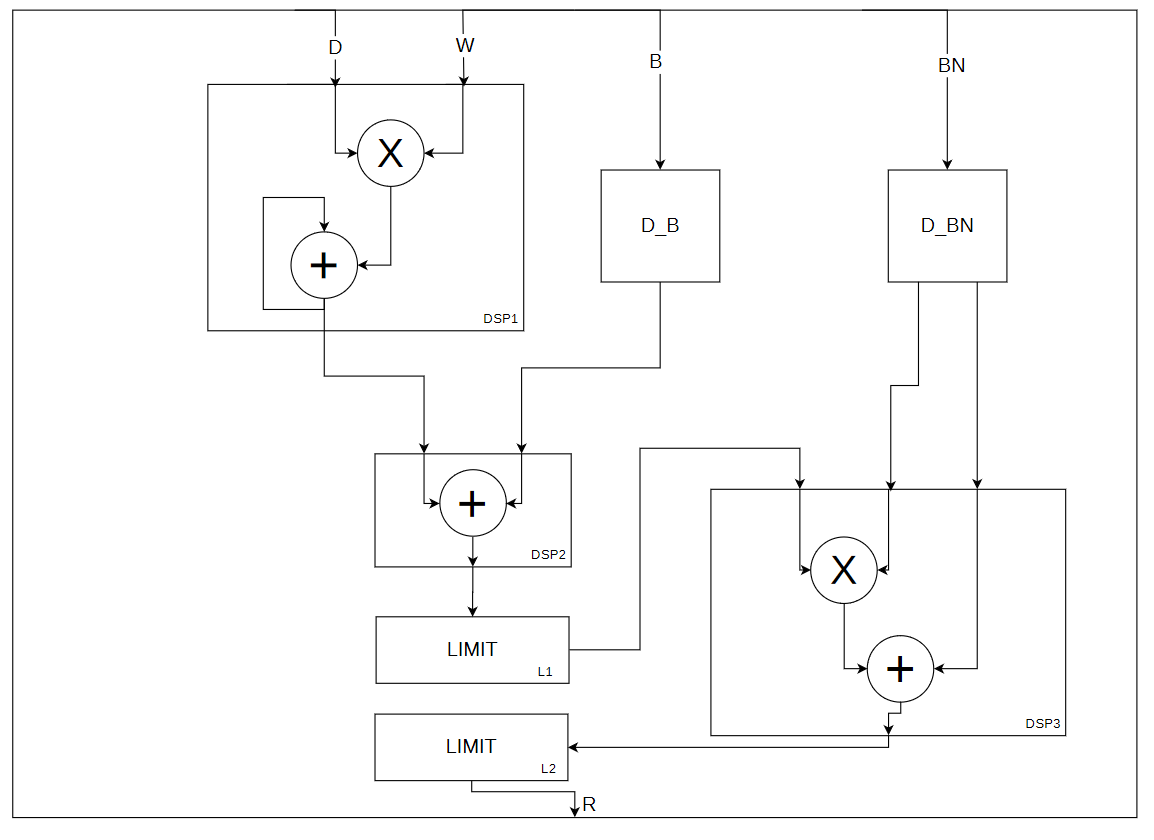
\includegraphics[width=0.9\linewidth]{images/PW_PU.png}
    \caption{Schemat \emph{PW\_PU} - akumulacja z mnożeniem realizowane przez \emph{DSP}. Bloki \emph{DSP2} oraz \emph{DSP3+L2} są opcjonalne zależne od konfiguracji.}
    \label{fig:pwpu}
\end{figure}




